%=======================================================================================================
% Ogmg Multigrid solver: Report
%=======================================================================================================
\documentclass[11pt]{article}

\usepackage[bookmarks=true]{hyperref}

% \input documentationPageSize.tex
\hbadness=10000 
\sloppy \hfuzz=30pt

\usepackage{calc}
% set the page width and height for the paper (The covers will have their own size)
\setlength{\textwidth}{7in}  
\setlength{\textheight}{9.5in} 
% here we automatically compute the offsets in order to centre the page
\setlength{\oddsidemargin}{(\paperwidth-\textwidth)/2 - 1in}
% \setlength{\topmargin}{(\paperheight-\textheight -\headheight-\headsep-\footskip)/2 - 1in + .8in }
\setlength{\topmargin}{(\paperheight-\textheight -\headheight-\headsep-\footskip)/2 - 1in -.2in }

\input homeHenshaw

\usepackage{amsmath}
\usepackage{amssymb}

\usepackage{verbatim}
\usepackage{moreverb}
\usepackage{graphics}    
\usepackage{epsfig}    
% \usepackage{calc}
% \usepackage{ifthen}
% \usepackage{float}
% \usepackage{fancybox}

\usepackage{makeidx} % index
\makeindex
\newcommand{\Index}[1]{#1\index{#1}}

\input{pstricks}\input{pst-node}

\begin{document}

% -----definitions-----

\newcommand{\ogen}{/home/henshaw/res/ogen}
\newcommand{\figures}{/home/henshaw/Overture/docFigures}
\newcommand{\automg}{/home/henshaw/papers/automg}
% \newcommand{\automg}{../automg}
\newcommand{\ogmgDir}{/home/henshaw/Overture/ogmg}
% \newcommand{\ogmgDir}{.}

\newcommand{\Ogen}{{Ogen}}
\newcommand{\Overture}{{Overture}}
\newcommand{\Ogmg}{{Ogmg}}
\newcommand{\figWidth}{.495\linewidth}
\newcommand{\clipfig}{}
\newcommand{\tablefontsize}{\normalsize}

\input wdhDefinitions.tex


%---------- Title Page for a Research Report----------------------------
\vspace{5\baselineskip}
\begin{flushleft}
{\Large
On Multigrid for Overlapping Grids \\
}
\vspace{3\baselineskip}
William D. Henshaw   \\                    
\vspace{2\baselineskip}
Centre for Applied Scientific Computing \\
Lawrence Livermore National Laboratory    \\
Livermore, CA, 94551   \\
henshaw@llnl.gov \\
http://www.llnl.gov/casc/people/henshaw \\
http://www.llnl.gov/casc/Overture\\
\vspace{2\baselineskip}
\today\\
\vspace{\baselineskip}
UCRL-MA-??????


\vspace{4\baselineskip}

\noindent{\bf Abstract:}
  We describe various aspects of solving elliptic boundary value problems
on overlapping grids.


We describe the Overlapping-Grid-MultiGrid-solver, \Ogmg, that can be used to obtain solutions 
to elliptic boundary value problems.
% on composite overlapping grids with the multigrid algorithm.  
\Ogmg~ solves problems in two and three space
dimensions on composite overlapping grids. 
Second and fourth-order accurate approximations are supported.
Given an overlapping grid generated from the \Ogen~  grid generator,
\Ogmg~  will generate the coarse grid multigrid levels using an automatic coarsening algorithm.
The equations on the coarse grids can be determined automatically using a Galerkin averaging
procedure.
The multigrid solution algorithm has been optimised for some commonly occuring problems such as
equations defined with the Laplace operator.
Smoothers include Red-Black, Jacobi, Gauss-Seidel, line-zebra and line-Jacobi.
\Ogmg~  is particularly efficient when a majority of the grid points belong to cartesian component grids;
this is often the case when grids become sufficiently fine.
The fourth-order accurate approximations are solved directly with multigrid (as opposed to using
a defect correction scheme). Convergence rates for the fourth-order approximations are often nearly as
good as the convergence rates for second-order discretizations.
Currently only scalar elliptic boundary value problems can be solved. 
\end{flushleft}

\vfill\eject
\tableofcontents
% \listoffigures

%---------- End of title Page for a Research Report


\vfill\eject
\section{Introduction}\index{multigrid}

\Ogmg~ is a multigrid solver for use with \Overture~\cite{overset96},\cite{OGES}.
\Ogmg~ can solve scalar elliptic problems
on overlapping grids. It has a variety of smoothers including
Red-Black, Jacobi, Gauss-Seidel and line smoothers. Second-order accurate and fourth-order
accurate approximations are supported.
A sparse direct or sparse iterative
solver such as GMRES can be used to solve the coarse grid equations --
the \Overture~ solver Oges is used for this purpose, thus allowing access to a variety of
sparse matrix solvers such as those available with PETSc\cite{PETSc}.

In the case of a general elliptic boundary value problem, 
the system of equations that \Ogmg~ solves are specified as a ``coefficient-array''
grid function. The coefficient array can be created using the Overture operator classes. 

% The user of Ogmg is responsible for creating these equations at all multigrid levels.
% The automatic generation of coarse grid equations by Galerkin averaging 
% is not yet implemented.

Ogmg has been specifically optimised for a class of commonly occuring problems. These
{\sl predefined} equations are 
\begin{alignat*}{3} \label{eq:predefined}
   \Delta u & = f &\qquad&  \mbox{laplaceEquation}  \\
   \grad\cdot( s(\xv) \grad) u & = f &\qquad&  \mbox{divScalarGradOperator} \\
   (I + c_0 \Delta) u & = f &\qquad&  \mbox{heatEquationOperator}  \\
  (I + s(x) \Delta) u & = f &\qquad&  \mbox{variableHeatEquationOperator}  \\
  (I + \grad\cdot( s(\xv) \grad)) u & = f &\qquad&  \mbox{divScalarGradHeatEquationOperator} 
\end{alignat*}
These equations are augmented with Dirichlet, Neumann or mixed boundary conditions.
The above equations can be solved more quickly and with less storage than if the same equation had been
defined through a general coefficient matrix.

\Ogmg~ starts with an overlapping grid constructured with the overlapping grid generator Ogen.
The coarse grids needed by the multigrid algorithm 
are automatically generated with a new coarsening algorithm. Very coarse grids
can be formed by relaxing the accuracy requirements for interpolation on the coarser grids and
allowing the overlap between grids to grow as the grids are coarsened.

The discrete approximations to the equations on the coarse grids are determined automatically
using a Galerkin averaging procedure from finer grids.

An adaptive smoothing algorithm is used to improve the convergence rate. The number of sub-smooths
performed on each component grid is adjusted to keep the residuals nearly the same.

Good multigrid convergence rates are usually obtained. 
\Ogmg~  is particularly efficient when a majority of the grid points belong to cartesian component grids;
this is often the case when grids become sufficiently fine.
The overall convergence rates has been significanty improved from the original fortran version of
the code~\cite{CGMG}. Some of the factors that led to this improved performance were
\begin{itemize}
  \item an adaptive smoothing algorithm that performs additional sub-smooths on component grids that 
        are converging slowly.
  \item generating the coarse grid equations through operator averaging improves the convergence rate.
  \item careful attention to boundary conditions (especially for Neumann boundary conditions and
    fourth-order accurate discretzations) can improve the convergence rate.
  \item using over-relaxation for Red-Black smoothers is very helpful, especially in 3D.
\end{itemize}

Ogmg does not yet efficiently handle the case of singular problems such as a Poisson equation
with all Neumann boundary conditions; in this case one must first determine the left null vector
to the discrete operator. 


\section{The multigrid algorithm for overlapping grids}\index{multigrid!overlapping grid algorithm}

Ogmg uses the standard defect correction algorithm. The implementation
on overlapping grids is relatively straight-forward. See the paper \cite{CGMG}
for further discussion.

\begin{itemize}
\item Typically Jacobi, red-black or line (zebra) smoothers are used.

\item The fine to coarse {\sl Restriction} operator is the {\it full weighting}
operator except at boundaries.

\item The coarse to fine Prolongation operator is second or fourth
order interpolation; second-order by default.

\item The {\bf cycle} chosen is either adaptive or can be fixed
to a desired one.
\end{itemize}


\begin{tabbing}
1234567890 \= 1234 \= 1234 \= 1234 \= 1234 \=  \kill  % define tabs
\> {\bf while} {\it not converged} {\bf do}                   \\
\>\>  smooth $\nu_1$ times or until the smoothing rate $> \eta$      \\
\>\>\>  $v_1 \gets S^{\nu_1} v_1$                                    \\
\>\>    form the defect and transfer to the coarser grid             \\
\>\>\>  $f_2 \gets R^{1\to2} ( f-A v_1) $                            \\
\>\>  ``solve'' the defect equation (at least to an
                ``accuracy'' of $\delta$) \\
\>\>\>    $A_2 v_2 \approx f_2$                                      \\
\>\>    correct the fine grid solution from the coarse grid solution \\
\>\>\>  $v_1 \gets v_1 + P^{2\to1} v_2 $                             \\
\>\>  smooth $\nu_2$ times or until the smoothing rate $> \eta$      \\
\>\>\>  $v_1 \gets S^{\nu_2} v_1$                                    \\
\> {\bf end while}
\end{tabbing}

The {\bf smoothing step} represented by the operator $S$ 
is a {\sl composite-smooth} where each grid in turn
is smoothed:
\begin{tabbing}
1234567890 \= 1234 \= 1234 \= 1234 \= 1234 \=  \kill  % define tabs
\> {\bf for } {\it each grid $g$ in a CompositeGrid} {\bf do}                   \\
\>\>  smooth grid g $\nu_g$ times       \\
\>\>  interpolate \\
\> {\bf end for}
\end{tabbing}
The smoother and the number of smooths may vary from component grid to
component grid. We try
to choose $n_g$, the number of smooths on each component grid, so that the
residual stays about the same size on each component grid. The approximate rule
we use is that
\[
    n_g \approx { \| \text{ residual on grid $g$} \| \over \min_g \| \text{residual on grid $g$} \| }
\]
The grid with the smallest residual will have $n_g=1$. 



\section{Black box multigrid features}

A new feature of Ogmg is the ability to take a problem defined on a CompositeGrid
with only one level and to automatically generate the information for coarser levels.
There are two key ingredients to making this work. The first is that we need to generate
the coarse grid coefficient matrices automatically. The second is to handle interpolation
points on the coarse grid which may or may not sit on interpolation points on the fine grid.

\subsection{Automatic coarsening algorithms}



\subsection{Operator averaging}


To generate a coarse grid operator from a fine grid operator we can
average the operator on the fine grid and then restrict the result
to the coarse grid.

Consider a 3 point stencil operator in one dimension. If we look at the stencil for
rows $i-1,i,i+1$ arranged in a matrix then we get
\[
   \begin{matrix}
   a_{i-1}u_{i-2} & b_{i-1}u_{i-1} & c_{i-1} u_i  & 0              & 0 \\
       0          & a_i u_{i-1}    & b_i u_i      & c_i u_{i+1}    & 0\\
       0          &       0        & a_{i+1} u_i  & b_{i+1}u_{i+1} & c_{i+1}u_{i+2} \\
    \end{matrix}
\]
If we replace row $i$ by the weighted average of rows $i-1,i,i+1$ with weights $\alpha$, $\beta$, $\alpha$
then we get the wide stencil
\[
   \begin{matrix}
     \alpha a_{i-1}u_{i-2} & 
         (\alpha b_{i-1}+\beta a_i)u_{i-1}  &
         (\alpha( c_{i-1} + a_{i+1}) + \beta b_i ) u_i &
         (\alpha b_{i+1}+\beta c_i)u_{i-1}  &
     \alpha c_{i+1}u_{i+2} 
    \end{matrix}
\]
If we distribute the values at point $i-1$ using $u_{i-1}=\half( u_{i-2}+u_i )$ and at point $i+1$
using $u_{i+1}=\half( u_{i+2}+u_i )$ then we have a wide stencil only defined at points
$i-2,i,i+2$.
\[
   \begin{matrix}
     ( \alpha(a_{i-1}+\half b_{i-1}) +\half\beta a_i) u_{i-2} & 
         &
         (\alpha( \half b_{i-1} + \half b_{i+1} + c_{i-1} + a_{i+1}) + \beta (b_i+\half a_i+\half c_i) ) u_i &
         &
     (\alpha( c_{i+1}\half b_{i+1}) + \half\beta c_i)u_{i+2} 
    \end{matrix}
\]

Typically we take $\alpha=\gamma=1/4$, and $\beta=1/2$.  In more than one space dimension we can
apply the above averaging procedure sequentially in each direction. 


Now consider a 5 point operator (we could also average 5 adjacent equations rather then 3)
\[
   \begin{matrix}
a_{i-1}u_{i-3}& b_{i-1}u_{i-2}& c_{i-1} u_{i-1}& d_{i-1} u_{i} & e_{i-1} u_{i+1} &  0              & 0 \\
    0         & a_i u_{i-2}   & b_i u_{i-1}    & c_i u_{i  }   & d_{i  } u_{i+1} & e_{i  } u_{i+2} & 0\\
    0         &       0       & a_{i+1} u_{i-1}& b_{i+1}u_{i}  & c_{i+1}u_{i+1}  & d_{i+1} u_{i+2} & e_{i+1} u_{i+3} \\
    \end{matrix}
\]
Averaging in a similar fashion we obtain a coarse grid operator
\[
   \begin{matrix}
    a_i^c u_{i-2}   & b_i^c u_{i-1}    & c_i^c u_{i}  & d_{i}^c u_{i+1} & e_{i}^c u_{i+2} \\
    \end{matrix}
\]
where
\begin{align*}
   a_i^c &= \half\alpha a_{i-1} \\  
   b_i^c &=  \alpha b_{i-1} + \beta a_i + \half \alpha a_{i-1}+
                \half( \alpha c_{i-1} + \beta b_i + \alpha a_{i+1} )      \\
   c_i^c &= \alpha d_{i-1} + \beta c_i +\alpha b_{i+1} +
               \half( \alpha c_{i-1} + \beta b_i + \alpha a_{i+1} ) +
               \half( \alpha e_{i-1} + \beta d_i + \alpha c_{i+1} ) \\
   d_i^c &=  \alpha d_{i+1} + \beta e_i +
              \half( \alpha e_{i-1} + \beta d_i + \alpha c_{i+1} ) +
               \half\alpha e_{i+1} \\
   e_i^c &= \half\alpha e_{i+1} \\  
\end{align*}


\subsubsection{Operator averaging at boundaries}

   At a boundary we will typically have a boundary condition such as a dirichlet, neumann or mixed boundary
condition. We need to decide how to average near the boundary and on the boundary or ghost line.

Ogmg is aware of two types of boundary conditions. These 'boundary conditions' actually
just indicate how the {\bf ghost line} should be updated. The condition {\tt extrapolation} indicates the 
ghost line is extrapolated and usually means that a dirichlet boundary condition is applied on
the boundary. The {\tt equation} boundary condition indicates that some equation is applied on
the ghost line; this is usually associated with a neumann or mixed boundary condition.

\begin{description}
  \item[dirichlet] : In this case we just impose a dirichlet BC in the coarse grid operator.
  \item[neumann] : (or neumann like condition) coarse grid operator. The coarse grid operator is
     obtained by distributing the fine grid ghost line equation to the coarser grid but not averaged
     in the tangential direction.
\[
   \begin{matrix}
     ( \alpha(a_{i}+\half b_{i}) +\half\beta a_i) u_{i-2} & 
         &
         (\alpha( b_i + c_i + a_i) + \beta (b_i+\half a_i+\half c_i) ) u_i &
         &
     (\alpha( c_i + \half b_i) + \half\beta c_i)u_{i+2} 
    \end{matrix}
\]
  \item[extrapolation] : coarse grid operator is also extrapolation.
  \item[equation] : ghost line has some equation on it. The coarse grid operator is obtained by
       averaging the ghostline equations (i.e. averaging is only done in the tangential directions).
\end{description}






{\bf Remark:} 
The coarse grid matrix $A^{2}$ can also be defined from the fine grid matrix $A^1$ using the prologation
and restriction operators
\[
     A^2 = R A^1 P
\]
The first step above where the rows were combined corresponds to premultiplying $A^1$
by $R$.
The second step where the values at points $i+1$ and $i+1$ were removed corresponds to the post-multiplication
by $P$.

Tables~(\ref{tab:operatorAveraging}-\ref{tab:operatorAveraging4}) 
compare the convergence results for Poisson's equation with 
dirichlet boundary conditions when using operator averaging to construct the coarse grid equations
to no operator averaging. The notation used to label the columns in defined 
at the start of section~\ref{sec:numericalResults}.
In this example the operator-averaged case is significantly better.
There was a negligible difference in CPU times between the two cases.

\renewcommand{\figWidth}{.495\linewidth}
\begin{figure}
\begin{center}
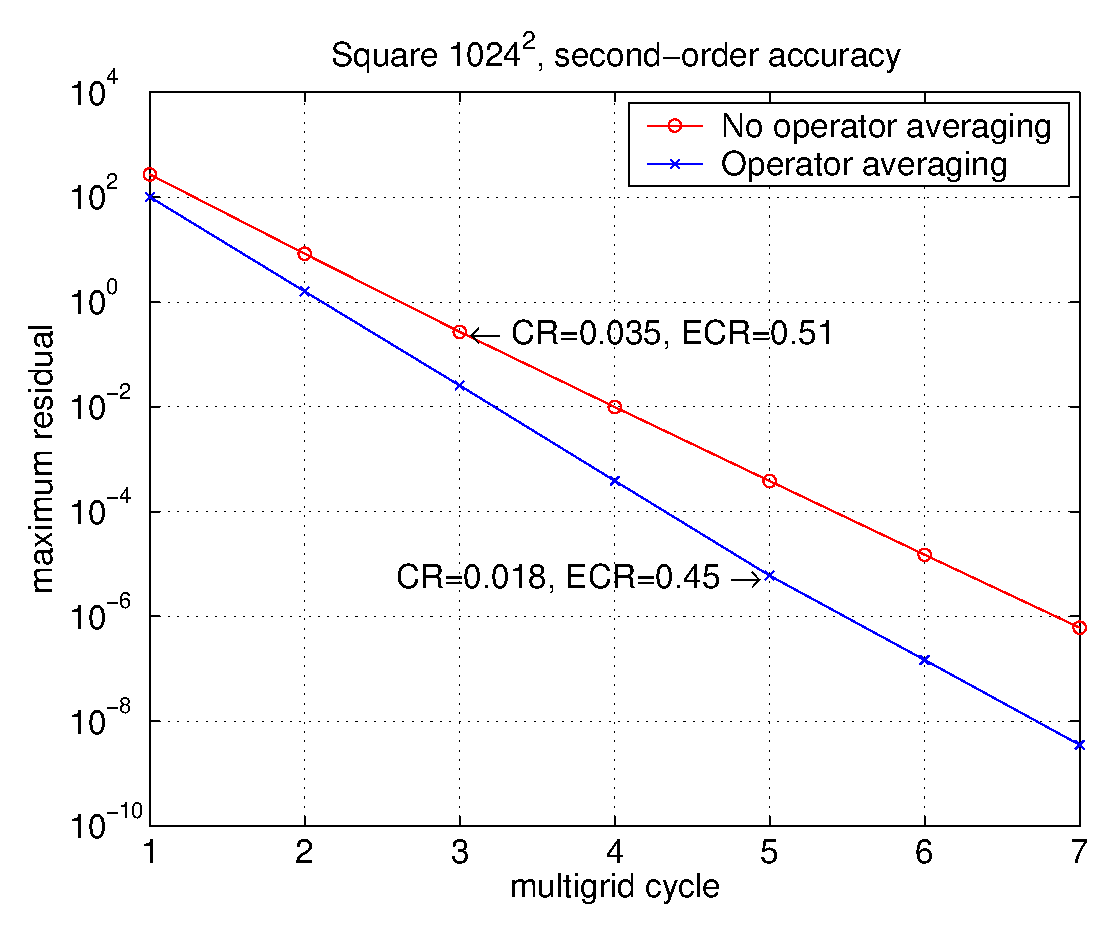
\epsfig{file=opAveComparison.eps,width=\figWidth}
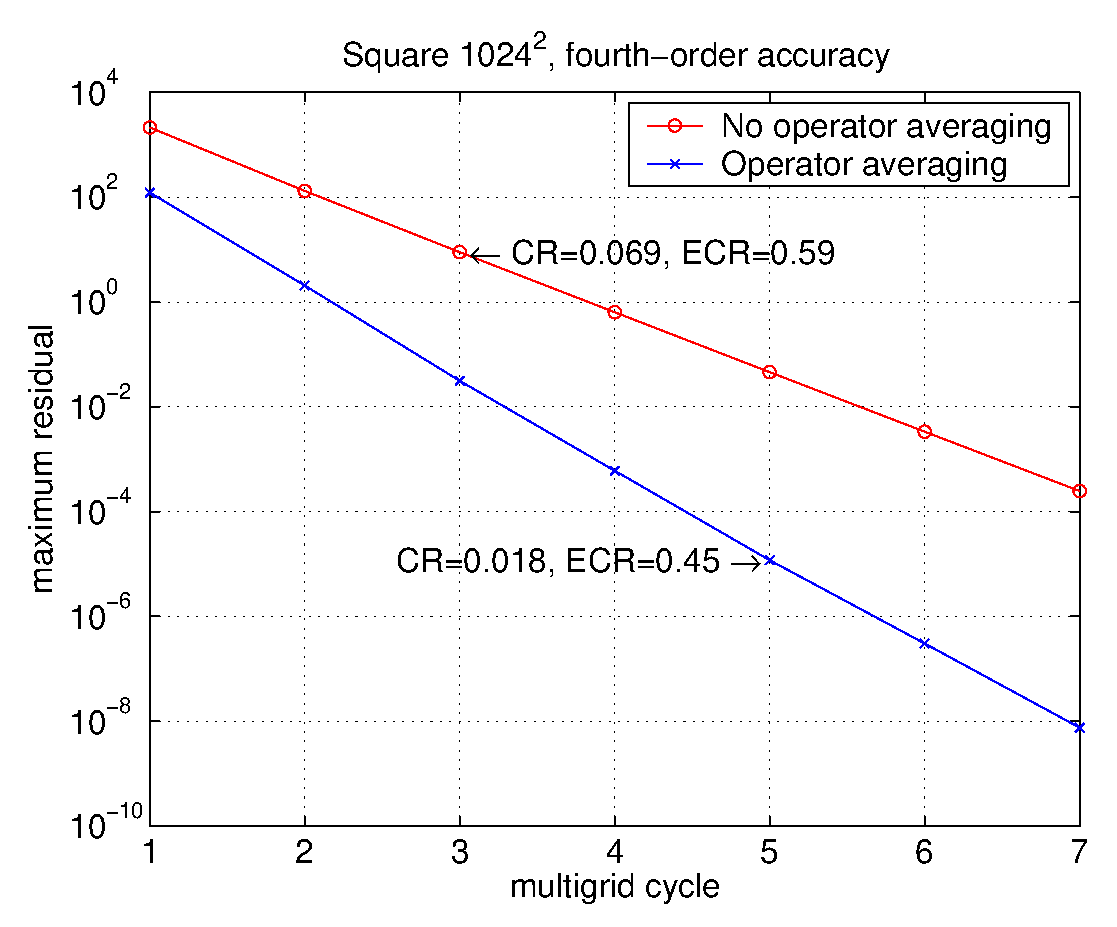
\epsfig{file=opAveComparison4.eps,width=\figWidth}\\
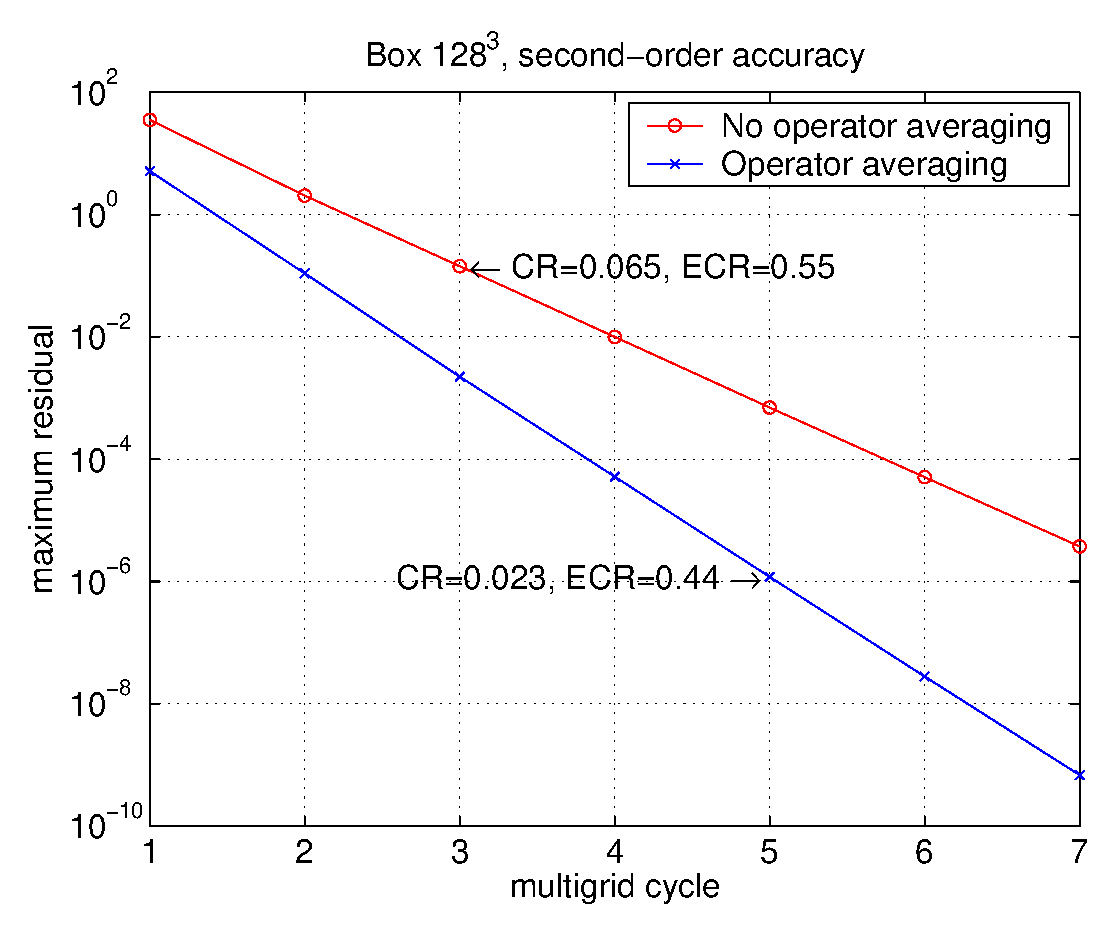
\epsfig{file=opAveComparison.box128.eps,width=\figWidth}
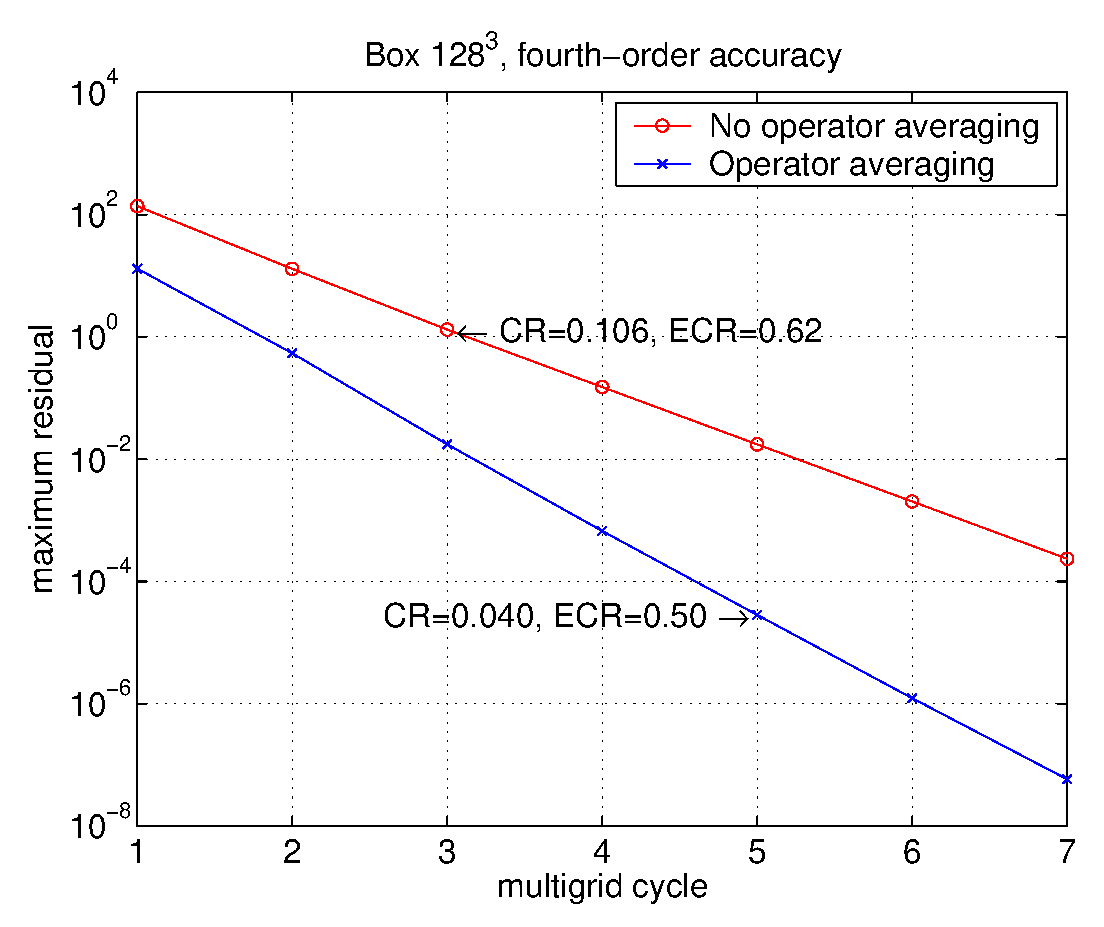
\epsfig{file=opAveComparison4.box128.eps,width=\figWidth}\\
\end{center}
\caption{The convergence rate is improved when the coarse grid operators are generated
with operator averaging. Results are shown for a V[2,1] cycle.}
\label{fig:opAveComparison}
\end{figure}


\begin{table}[hbt]
\begin{center}
\begin{tabular}{|c|c|c|c|c|} \hline 
 \multicolumn{5}{|c|}{With Operator Averaging}\\   \hline 
 $i$   & res      & rate    &  WU    & ECR  \\   \hline 
 $ 1$  & $ 1.4e+02$ & $0.036$ & $ 5.0$ & $0.52$ \\ 
 $ 2$  & $ 3.4e+00$ & $0.024$ & $ 5.0$ & $0.48$ \\ 
 $ 3$  & $ 9.3e-02$ & $0.027$ & $ 5.0$ & $0.49$ \\ 
 $ 4$  & $ 2.5e-03$ & $0.027$ & $ 5.0$ & $0.49$ \\ 
 $ 5$  & $ 7.1e-05$ & $0.028$ & $ 5.0$ & $0.49$ \\ 
 $ 6$  & $ 2.0e-06$ & $0.029$ & $ 5.0$ & $0.49$ \\ 
 $ 7$  & $ 5.9e-08$ & $0.029$ & $ 5.0$ & $0.50$ \\ 
\hline 
\end{tabular} \qquad
\begin{tabular}{|c|c|c|c|c|} \hline 
 \multicolumn{5}{|c|}{Without Operator Averaging}\\   \hline 
 $i$   & res      & rate    &  WU    & ECR  \\   \hline 
 $ 1$  & $ 2.3e+02$ & $0.054$ & $ 5.0$ & $0.56$ \\ 
 $ 2$  & $ 9.4e+00$ & $0.041$ & $ 5.0$ & $0.53$ \\ 
 $ 3$  & $ 5.2e-01$ & $0.055$ & $ 5.0$ & $0.56$ \\ 
 $ 4$  & $ 2.9e-02$ & $0.056$ & $ 5.0$ & $0.57$ \\ 
 $ 5$  & $ 1.7e-03$ & $0.058$ & $ 5.0$ & $0.57$ \\ 
 $ 6$  & $ 1.1e-04$ & $0.065$ & $ 5.0$ & $0.58$ \\ 
 $ 7$  & $ 7.4e-06$ & $0.067$ & $ 5.0$ & $0.58$ \\ 
\hline 
\end{tabular}\\
\end{center}
\caption{Second-order accuracy. Left: operator averaging. Right: no operator averaging. Multigrid convergence rates, 5 levels, smoother rb[2,1]. Grid square256, trigonometric solution.}
\label{tab:operatorAveraging} 
\end{table}


\begin{table}[hbt]
\begin{center}
\begin{tabular}{|c|c|c|c|c|} \hline 
 \multicolumn{5}{|c|}{With Operator Averaging}\\   \hline 
 $i$   & res      & rate    &  WU    & ECR  \\   \hline 
 $ 1$  & $ 3.0e+02$ & $0.048$ & $ 5.1$ & $0.55$ \\ 
 $ 2$  & $ 1.4e+01$ & $0.046$ & $ 5.1$ & $0.54$ \\ 
 $ 3$  & $ 7.0e-01$ & $0.051$ & $ 5.1$ & $0.55$ \\ 
 $ 4$  & $ 3.6e-02$ & $0.051$ & $ 5.1$ & $0.56$ \\ 
 $ 5$  & $ 1.9e-03$ & $0.052$ & $ 5.1$ & $0.56$ \\ 
 $ 6$  & $ 9.7e-05$ & $0.052$ & $ 5.1$ & $0.56$ \\ 
 $ 7$  & $ 5.1e-06$ & $0.053$ & $ 5.1$ & $0.56$ \\ 
\hline 
\end{tabular} \qquad
\begin{tabular}{|c|c|c|c|c|} \hline 
 \multicolumn{5}{|c|}{Without Operator Averaging}\\   \hline 
 $i$   & res      & rate    &  WU    & ECR  \\   \hline 
 $ 1$  & $ 9.4e+02$ & $0.111$ & $ 5.1$ & $0.65$ \\ 
 $ 2$  & $ 8.8e+01$ & $0.094$ & $ 5.1$ & $0.63$ \\ 
 $ 3$  & $ 9.8e+00$ & $0.111$ & $ 5.1$ & $0.65$ \\ 
 $ 4$  & $ 1.2e+00$ & $0.120$ & $ 5.1$ & $0.66$ \\ 
 $ 5$  & $ 1.4e-01$ & $0.122$ & $ 5.1$ & $0.66$ \\ 
 $ 6$  & $ 1.8e-02$ & $0.124$ & $ 5.1$ & $0.66$ \\ 
 $ 7$  & $ 2.2e-03$ & $0.126$ & $ 5.1$ & $0.66$ \\ 
\hline 
\end{tabular}\\
\end{center}
\caption{Fourth-order accuracy. Left: operator averaging. Right: no operator averaging. Multigrid convergence rates, 5 levels, smoother rb[2,1]. Grid square256.order4, trigonometric solution.}
\label{tab:operatorAveraging4} 
\end{table}


% -----------------------------------------------------------
\section{Smoothing overlapping grids}

There are a few issues that must be addressed when smoothing an overlapping grid.
Some care must be taken to ensure that the composite-smooth operator (a smoothing step
over all component grids) retains similiar smoothing rates to that of a smoother for a 
single component grid. The underlying principle for smoothing an overlapping
grid is that the defect after smoothing should be smooth enough to be represented 
on the next coarser levels.





\bibliography{\homeHenshaw/papers/henshaw}
\bibliographystyle{siam}

\printindex

\end{document}




